%%%%%%%%%%%%%%%%%%%%%%%%%%%%%%%%%%%%%%%%%
%
% This template has been downloaded from:
% http://www.LaTeXTemplates.com
%
% License:
% CC BY-NC-SA 3.0 (http://creativecommons.org/licenses/by-nc-sa/3.0/)
%
%%%%%%%%%%%%%%%%%%%%%%%%%%%%%%%%%%%%%%%%%

%----------------------------------------------------------------------------------------
%	PACKAGES AND THEMES
%----------------------------------------------------------------------------------------

\documentclass{beamer}

\mode<presentation> {

% The Beamer class comes with a number of default slide themes
% which change the colors and layouts of slides. Below this is a list
% of all the themes, uncomment each in turn to see what they look like.

%\usetheme{default}
%\usetheme{AnnArbor}
%\usetheme{Antibes}
%\usetheme{Bergen}
%\usetheme{Berkeley}
%\usetheme{Berlin}
%\usetheme{Boadilla}
%\usetheme{CambridgeUS}
%\usetheme{Copenhagen}
%\usetheme{Darmstadt}
%\usetheme{Dresden}
%\usetheme{Frankfurt}
%\usetheme{Goettingen}
%\usetheme{Hannover}
%\usetheme{Ilmenau}
%\usetheme{JuanLesPins}
%\usetheme{Luebeck}
\usetheme{Madrid}
%\usetheme{Malmoe}
%\usetheme{Marburg}
%\usetheme{Montpellier}
%\usetheme{PaloAlto}
%\usetheme{Pittsburgh}
%\usetheme{Rochester}
%\usetheme{Singapore}
%\usetheme{Szeged}
%\usetheme{Warsaw}

% As well as themes, the Beamer class has a number of color themes
% for any slide theme. Uncomment each of these in turn to see how it
% changes the colors of your current slide theme.

%\usecolortheme{albatross}
%\usecolortheme{beaver}
%\usecolortheme{beetle}
%\usecolortheme{crane}
%\usecolortheme{dolphin}
%\usecolortheme{dove}
%\usecolortheme{fly}
%\usecolortheme{lily}
%\usecolortheme{orchid}
%\usecolortheme{rose}
%\usecolortheme{seagull}
%\usecolortheme{seahorse}
%\usecolortheme{whale}
\usecolortheme{wolverine}

%\setbeamertemplate{footline} % To remove the footer line in all slides uncomment this line
%\setbeamertemplate{footline}[page number] % To replace the footer line in all slides with a simple slide count uncomment this line

%\setbeamertemplate{navigation symbols}{} % To remove the navigation symbols from the bottom of all slides uncomment this line
}


\usepackage{graphicx} % Allows including images
\usepackage{svg}		%Allows including vector graphics
\usepackage{booktabs} % Allows the use of \toprule, \midrule and \bottomrule in tables
\graphicspath{ {./images/} }

\usepackage{flowchart}

\usepackage{tikz} % allows to use tikz graphics
\usetikzlibrary{shapes,snakes}
\usetikzlibrary{shapes.misc, shapes.arrows}
\usetikzlibrary{calc, matrix,chains,scopes,positioning,arrows,fit}


\newenvironment<>{varblock}[2][.9\textwidth]{%
  \setlength{\textwidth}{#1}
  \begin{actionenv}#3%
    \def\insertblocktitle{#2}%
    \par%
    \usebeamertemplate{block begin}}
  {\par%
    \usebeamertemplate{block end}%
  \end{actionenv}}
  

%----------------------------------------------------------------------------------------
%	TITLE PAGE
%----------------------------------------------------------------------------------------

\title[Software Engineering Project]{Software Engineering Project} % The short title appears at the bottom of every slide, the full title is only on the title page

\author{Cornell\`{a}, Garcia, Kozlovskis, Pak} % Your name
\institute[VIBOT 8] % Your institution as it will appear on the bottom of every slide, may be shorthand to save space
{
University of Burgundy \\ % Your institution for the title page
\medskip

}
\date{7th January 2014} % Date, can be changed to a custom date
\logo{%
  %\makebox[0.95\paperwidth]{
    
\includegraphics[height=0.8cm,keepaspectratio]{ubLogo}

  %}
}

\begin{document}

\begin{frame}
\titlepage % Print the title page as the first slide
%\logo{\includegraphics[height=0.8cm]{ub_logo}\vspace{220pt}}
\end{frame}

\begin{frame}
\frametitle{Outline}
%\tableofcontents[sectionstyle=show]

	\begin{itemize}
		\item Tools and resources
		\item Methodology
		\item C++ implementation
		\item Matlab implementation	
	\end{itemize}
\end{frame}

\section{Tools and resources}
\begin{frame}
\frametitle{Tools and resources}
\begin{columns}

\begin{column}{6cm}

	\begin{varblock}[5.8cm]{IDE}
	\begin{itemize}
	\item
	Qt 5.1 with OpenGL
	\item
	Matlab 2013Ra
	\end{itemize}
	\end{varblock}
	
	\begin{varblock}[5.8cm]{Group meetings and coordination}
	\begin{itemize}
	\item
	Trello
	\item
	Git and Bitbucket
	\end{itemize}
	\end{varblock}
	
	\begin{varblock}[5.8cm]{Database}
	\begin{itemize}
	\item
	MySQL Server 5.6
	\item
	PostgreSQL
	\end{itemize}
	\end{varblock}
\end{column}
	
\begin{column}{6cm}
	\begin{figure}[r]
	\centering
	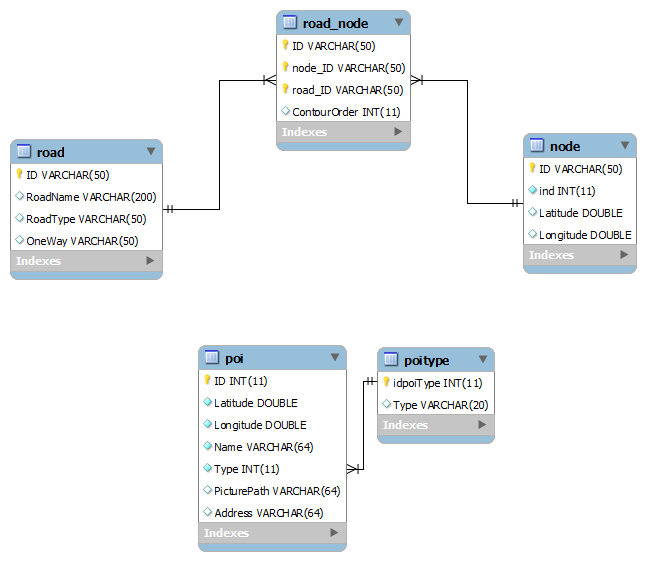
\includegraphics[width=1\textwidth]{big_schneider}
	\end{figure}
\end{column}
	
	
\end{columns}
\end{frame}

\section{C++ Implementation}
\begin{frame}
\frametitle{C++ Implementation}
\begin{itemize}
\item
Main Structure:

\begin{figure}[h]
\centering
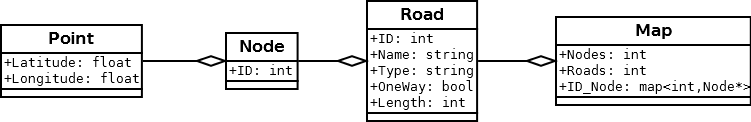
\includegraphics[width=0.8\textwidth]{main_structure}
\end{figure}

\item
Loaded in memory through QMYSQL Driver

\item
Displayed using GL\_STRIPES of OpenGL

\item
Creation of a map of ID\_Node* because of the complexity
	\begin{itemize}
	\item
	Avoiding Queries
	\item
	Avoiding double loops
	\end{itemize}
\end{itemize}
\end{frame}

\begin{frame}
\frametitle{C++: Dijkstra's algorithm}
\begin{itemize}
\item
Other kind of algorithms:
	\begin{itemize}
	\item
	Bellman-Ford and SPFA
	\item
	Jonhson's algorithm
	\item
	Floyd-Warshall algorithm
	\item
	Dijkstra's algorithm
	\end{itemize}

\item
Why? Performs better with non negative values

\item
How it works?
	\begin{enumerate}
	\item
	Initialize D to 0 in the diagonal and $\infty$ in non connected nodes
	\item
	Suppose that $a = x$ (current node)
	\item
	Check all adjacent nodes of a except the ones that are marked
	\item
	If $(D_{i}�> D_{a}�+ d(a, v_{i}))$ then, $D_{i}�= D_{a}�+ d(a, v_{i})$
	\item
	Marked as completed the node a
	\item
	We take as next current node the smaller in D
	\item
	Go back to step 3 until there are nodes not marked
	\end{enumerate}

\end{itemize}
\end{frame}

\begin{frame}
\frametitle{C++: Adjacency Matrix}
\begin{itemize}
\item
Sparse Matrix of the Euclidean distance between nodes (Eigen library)
\end{itemize}


\begin{columns}
\begin{column}{3cm}

\begin{table}
\footnotesize
\tabcolsep=0.11cm
\begin{tabular}{| c | c | c | c | c |}
\hline
0 & 3 & 0 & 0 & 0 \\ \hline
22 & 0 & 0 & 0 & 17 \\ \hline
7 & 5 & 0 & 1 & 0 \\ \hline
0 & 0 & 0 & 0 & 0 \\ \hline
0 & 0 & 14 & 0 & 8 \\
\hline
\end{tabular}
\end{table}
\footnotesize
Results measured under
Debug mode and dependent 
on the performance of each
processor

\end{column}
\begin{column}{6cm}

\begin{table}
\footnotesize
\tabcolsep=0.11cm
\begin{tabular}{|l|r|r|r|r|r|r|r|r|}
\hline
Values: & 22 & 7 & 3 & 5 & 14 & 1 & 17 & 8 \\ \hline
InnerIndices: & 1 & 2 & 0 & 2 & 4 & 2 & 1 & 4 \\
\hline
\end{tabular}
\end{table}

\begin{figure}[h]
\centering
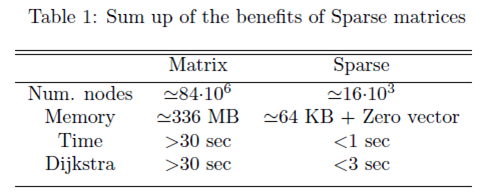
\includegraphics[width=0.9\textwidth]{sparse_benefits}
\end{figure}

\end{column}
\end{columns}

\end{frame}

\begin{frame}
\frametitle{Route path}

\begin{columns}
	\begin{column}{7cm}
		\begin{itemize}
		\item
		Functions:
			\begin{itemize}
			\item
			Path calculation
			\item
			Distance and time
			\item
			Export
			\end{itemize}
		\item
		General case:\\
		\scriptsize
		Same road $\rightarrow$ NO $\rightarrow$ $Angle<180$ $\rightarrow$ Right \\
		Same road $\rightarrow$ NO $\rightarrow$ $Angle>180$ $\rightarrow$ Left \\
		Same road $\rightarrow$ YES $\rightarrow$ Distance \\
		\end{itemize}
	\end{column}
	
	\begin{column}{6cm}
	\begin{figure}[h]
	\centering
	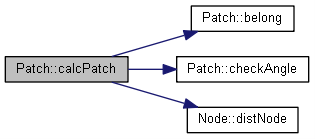
\includegraphics[width=0.7\textwidth]{route_path}
	\setbeamerfont{caption name}{size=\tiny}
	\caption{{\tiny Functions involved in the 
	route path calculation}}
	\end{figure}
	
	\begin{figure}[h]
	\centering
	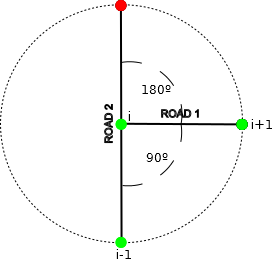
\includegraphics[width=0.5\textwidth]{angle}
	\setbeamerfont{caption name}{size=\tiny}
	\caption{{\tiny Example of road intersection}}
	\end{figure}
	\end{column}
\end{columns}
\end{frame}

\begin{frame}
\frametitle{Graphical User Interface (C++)}

\begin{figure}[r]
\centering
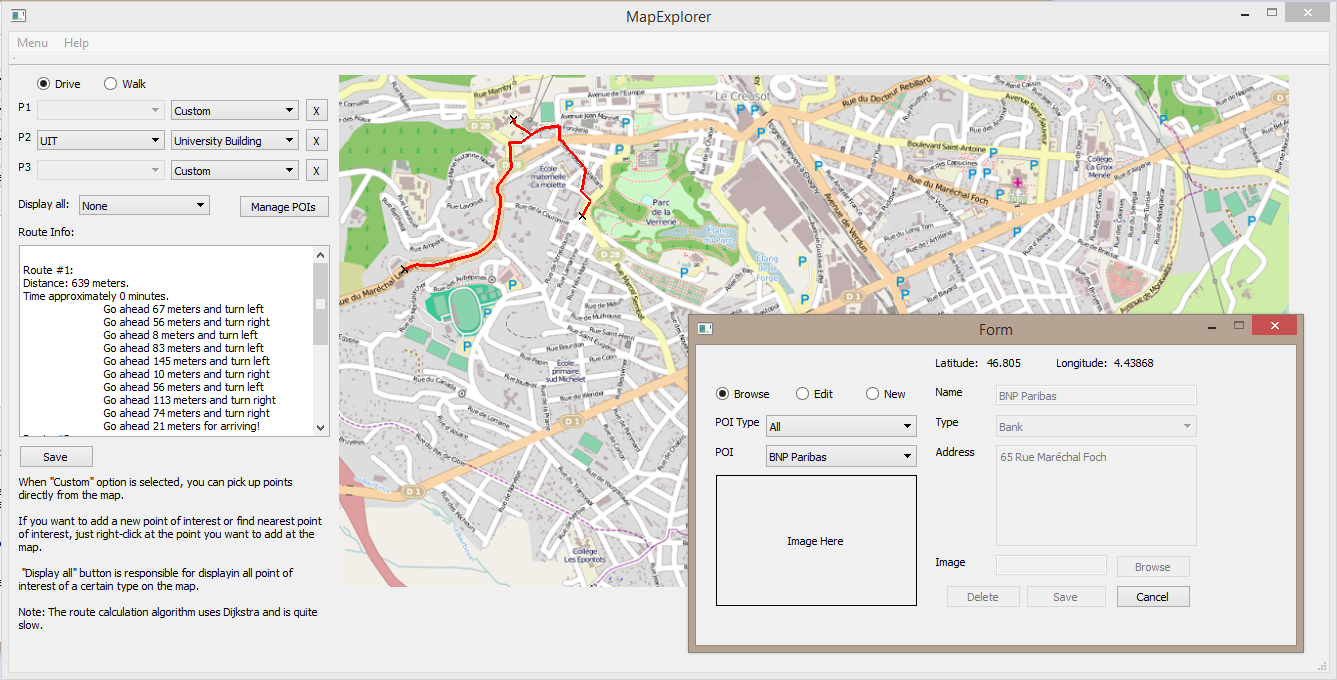
\includegraphics[width=1\textwidth]{cppgui}
\end{figure}

\end{frame}

\begin{frame}
\frametitle{Normalization and displaying}

\begin{itemize}
\item Geographic coordinates (latitude, longitude)
\item OpenGL (x,y)
	\begin{itemize}
	\item Map Texture
	\item glViewport, glOrtho and Qt Widget's size
	\end{itemize}
\item QGLWidget
\end{itemize}
\end{frame}

\begin{frame}
\frametitle{Route selection}

\begin{columns}
\begin{column}{6cm}
\begin{itemize}
\item Point from the map
\item Point of interest
\item Nearest Point of interest
\end{itemize}

\begin{figure}[h!]
\centering
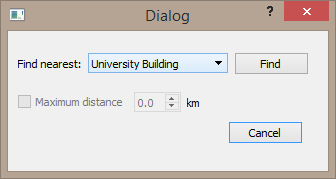
\includegraphics[width=0.8\textwidth]{cppnearest}
\caption*{Find nearest}
\end{figure}
\quad
\end{column}

\begin{column}{6cm}
\begin{figure}[h!]
\centering
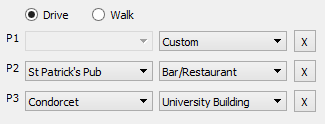
\includegraphics[width=0.8\textwidth]{cpprouteselection}
\caption*{Route selection interface}
\end{figure}

\begin{figure}[h!]
\centering
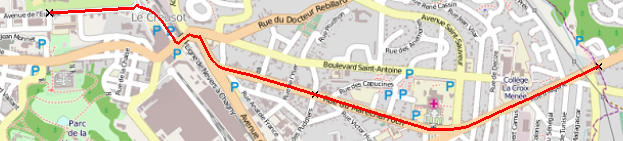
\includegraphics[width=1\textwidth]{cpproute}
\caption*{Route output}
\end{figure}

\end{column}
\end{columns}
\end{frame}

\begin{frame}
\frametitle{POI Management}
\framesubtitle{Add, modify and delete points of interest}

\begin{figure}[h!]
\centering
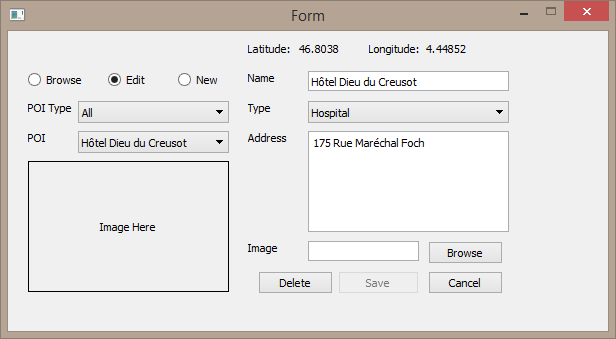
\includegraphics[width=0.8\textwidth]{cpppoi}
\end{figure}

\end{frame}

\section{Matlab implementation}
\begin{frame}
\frametitle{Matlab implementation}
\framesubtitle{Getting the data}
	\begin{itemize}
		\item Implemented database: PostgreSQL
		\item Same schema
		\item Cell matrix to data structure?
	\end{itemize}
\end{frame}

\begin{frame}
\frametitle{Matlab implementation}
\framesubtitle{Data Structure}
	\begin{itemize}
		\item Objects of 4 classes were constructed. 
		\item No pointers in Matlab.
		\item Solution: handle classes.
	\end{itemize}
	
	\begin{figure}[!h]
		\centering
			\begin{tikzpicture}[node distance=5mm,
			terminal/.style={
			% The shape:
			rectangle,
			minimum size=6mm,
			% The rest
			very thick,draw=black!50,
			top color=white,bottom color=black!15,
			font=\ttfamily}]
			
			\node (Node) [terminal] {Node};
			\node (ArrNode) [terminal,right=of Node] {ArrayNodes};
			\node (Road) [terminal,right=of ArrNode] {Road};
			\node (Map) [terminal,right=of Road] {Map (Array of Roads)};
			\path
			(Node) edge[-latex] (ArrNode) % simple edges
			(ArrNode) edge[-latex] (Road)
			(Road) edge[-latex] (Map);
			
			\end{tikzpicture}
		\caption{Simplified diagram of relationship of a classes}
	\end{figure}
\end{frame}

\begin{frame}
\framesubtitle{Data Structure}
	\begin{itemize}
		\item Created objects can be saved in .MAT files
		\item Queries were made only once.
		\item No need to recreate object on each program start
	\end{itemize}
\end{frame}

\begin{frame}
\frametitle{Matlab implementation}
\framesubtitle{The shortest path}
	\begin{itemize}
		\item Dijkstra's algorithm
		\item Determine the window on which the closest nodes and projections will be searched.
		\item Find the closest node on determined window.
		\item Find the closest projection (if possible) on the same window.
		\item Update the adjacency matrix according shortest distance.
	\end{itemize}
\begin{figure}[!h]
\centering
\begin{tikzpicture}[
	%	style def
    scale=0.6,
    important line/.style={thick},
    every node/.style={color=black}
    ]
	
	% demo connection of nodes
	\draw[important line] (0,1) coordinate (a1) -- (1,1.5) coordinate (a2) -- (3,2) coordinate (a3) -- (4,2) coordinate (a4);
	\draw[important line] (0,2.2)coordinate (C2) -- (1,2.5) coordinate (D) -- (2,3) coordinate (E) -- (2.5, 4.5) coordinate (F);
	\draw[important line] (a2)--(D) ;
	\draw[important line] (E)--(1,4) coordinate (G) -- (0,4.5) coordinate (H);
    \draw[important line] (3.5,4.5)coordinate (I) -- (3.4,3) coordinate (J)  --  (4,2.5) coordinate (K) ;
    \fill[black] 
        		 (a1) circle (2pt)
    			 (a2) circle (2pt)
    			 (a3) circle (2pt)
    			 (a4) circle (2pt)
    			 (C2) circle (2pt)
    			 (D) circle (2pt)
    			 (E) circle (2pt)
    			 (F) circle (2pt)
    			 (G) circle (2pt)
    			 (H) circle (2pt)
    			 (I) circle (2pt)
    			 (J) circle (2pt)
    			 (K) circle (2pt);
    %circle representing user input			 
    \fill[red] (2.6,2.5) circle (3pt) node[above] {$?$};
\end{tikzpicture}
\begin{tikzpicture}[
	%	style def
    scale=0.6,
    important line/.style={thick},
    every node/.style={color=black}
    ]
	
	% demo connection of nodes
	\draw[important line] (0,1) coordinate (a1) -- (1,1.5) coordinate (a2) -- (3,2) coordinate (a3) -- (4,2) coordinate (a4);
	\draw[important line] (0,2.2)coordinate (C2) -- (1,2.5) coordinate (D) -- (2,3) coordinate (E) -- (2.5, 4.5) coordinate (F);
	\draw[important line] (a2)--(D) ;
	\draw[important line] (E)--(1,4) coordinate (G) -- (0,4.5) coordinate (H);
    \draw[important line] (3.5,4.5)coordinate (I) -- (3.4,3) coordinate (J)  --  (4,2.5) coordinate (K) ;
    \fill[black] 
        		 (a1) circle (2pt)
    			 (a2) circle (2pt)
    			 (a3) circle (2pt)
    			 (a4) circle (2pt)
    			 (C2) circle (2pt)
    			 (D) circle (2pt)
    			 (E) circle (2pt)
    			 (F) circle (2pt)
    			 (G) circle (2pt)
    			 (H) circle (2pt)
    			 (I) circle (2pt)
    			 (J) circle (2pt)
    			 (K) circle (2pt);
    %circle representing user input			 
    \fill[red] (2.6,2.5) coordinate(user) circle (2pt) ;
    			     

    \draw[important line, blue] (user) -- (a3);
    \draw[important line, blue] (user) -- (E);
    \draw[important line, blue] (user) -- (J);
    %connecting closest nodes
        %circle representing user input			 
        \fill[red] (user) circle (3pt) node[above] {$?$};
        
    %square window line (dashed)
    \draw[important line, black, dashed] (2.6-0.9,2.5-0.9) -- (2.6-0.9,2.5+0.9) -- (2.6+0.9,2.5+0.9) -- (2.6+0.9,2.5-0.9) -- (2.6-0.9,2.5-0.9);
    
\end{tikzpicture}
\begin{tikzpicture}[
	%	style def
    scale=0.6,
    important line/.style={thick},
    every node/.style={color=black}
    ]
	
	% demo connection of nodes
	\draw[important line] (0,1) coordinate (a1) -- (1,1.5) coordinate (a2) -- (3,2) coordinate (a3) -- (4,2) coordinate (a4);
	\draw[important line] (0,2.2)coordinate (C2) -- (1,2.5) coordinate (D) -- (2,3) coordinate (E) -- (2.5, 4.5) coordinate (F);
	\draw[important line] (a2)--(D) ;
	\draw[important line] (E)--(1,4) coordinate (G) -- (0,4.5) coordinate (H);
    \draw[important line] (3.5,4.5)coordinate (I) -- (3.4,3) coordinate (J)  --  (4,2.5) coordinate (K) ;
    \fill[black] 
        		 (a1) circle (2pt)
    			 (a2) circle (2pt)
    			 (a3) circle (2pt)
    			 (a4) circle (2pt)
    			 (C2) circle (2pt)
    			 (D) circle (2pt)
    			 (E) circle (2pt)
    			 (F) circle (2pt)
    			 (G) circle (2pt)
    			 (H) circle (2pt)
    			 (I) circle (2pt)
    			 (J) circle (2pt)
    			 (K) circle (2pt);
   %circle representing user input			 
    \fill[red] (2.6,2.5) coordinate(user) circle (2pt) ;
    			     
	%connecting closest nodes
    \draw[important line, blue] (user) -- (a3);
    \draw[important line, blue] (user) -- (E);
    \draw[important line, blue] (user) -- (J);
    % projection
    \draw[important line, green] (user) -- (2.73, 1.95) coordinate (intersect);
    \fill[black] (intersect) circle (2pt) ;
    
    \draw[important line, green, ] (intersect)+(-0.14,0.07) node[scale = 0.6, minimum size=0.1cm,draw,green, rotate =14]{};
    %circle representing user input			 
    \fill[red] (user) circle (3pt) node[above] {$?$};
    \draw[important line] (a1) -- (a2) -- (a3) -- (a4);   
    
    %square window line (dashed)
    \draw[important line, black, dashed] (2.6-0.9,2.5-0.9) -- (2.6-0.9,2.5+0.9) -- (2.6+0.9,2.5+0.9) -- (2.6+0.9,2.5-0.9) -- (2.6-0.9,2.5-0.9);	 
\end{tikzpicture}
\caption{Finding the shortest point/projection for the random point on window domain}
\end{figure}
	
\end{frame}

\begin{frame}
\frametitle{Graphical User Interface (GUI)}
\begin{figure}[r]
\centering
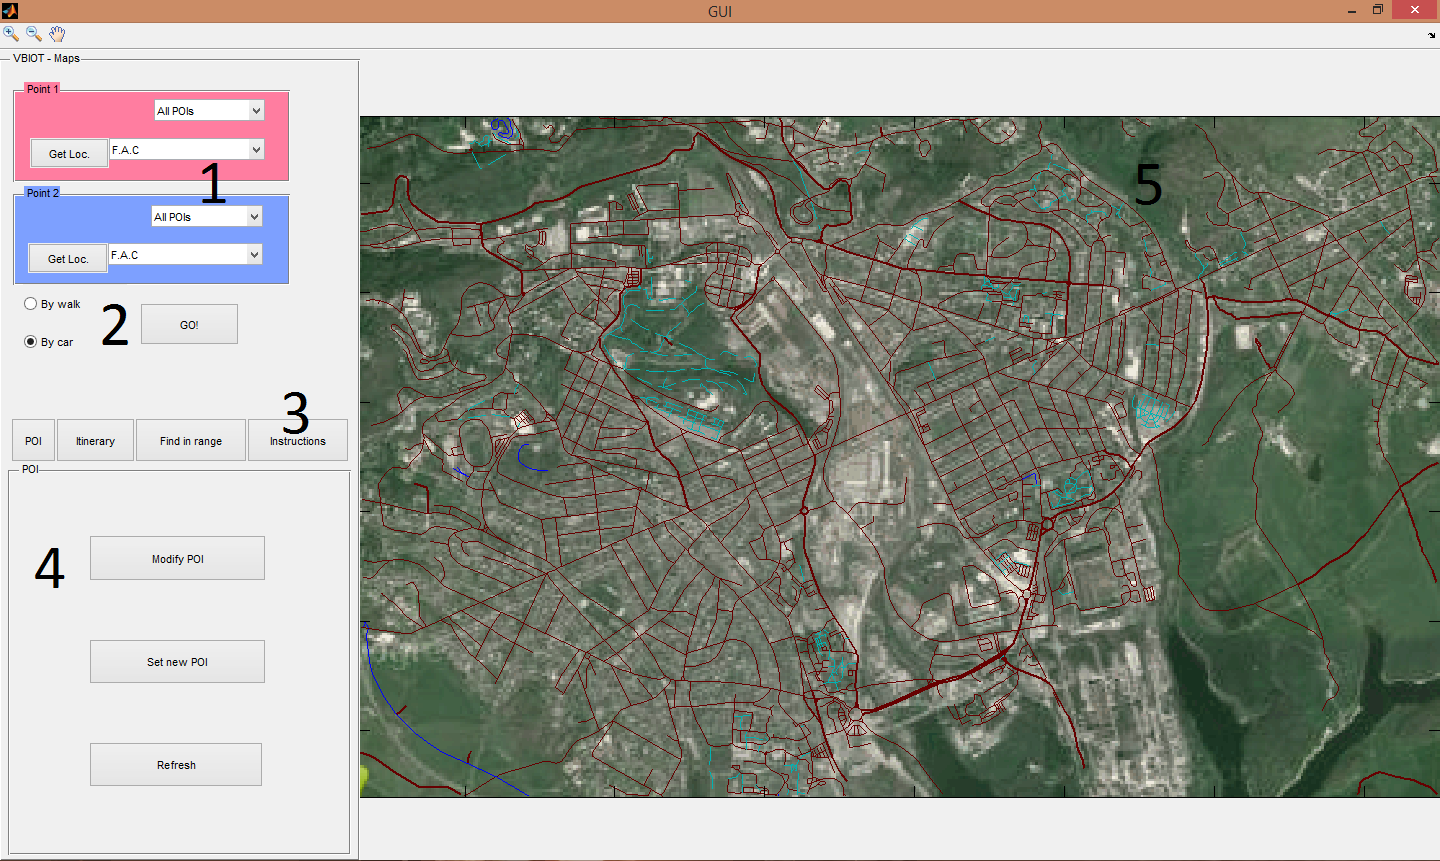
\includegraphics[width=1\textwidth]{gui}
\end{figure}
\end{frame}

\begin{frame}
\frametitle{Insertion of points}
\begin{columns}
	\begin{column}{6cm}
	\begin{itemize}
	\item
	Point from a list
	\item
	Filter by class
	\item
	Get Location from the map
	\item
	Walk / Car
	\item
	GO!
	\end{itemize}
	\end{column}
	
	\begin{column}{6cm}
	\begin{figure}[h]
	\centering
	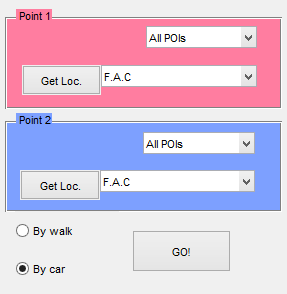
\includegraphics[width=0.8\textwidth]{gui_1}
	\end{figure}
	\end{column}
\end{columns}
\end{frame}

\begin{frame}
\frametitle{Manipulating Points of interest}

\begin{tikzpicture}[>=stealth, thick]
\node (A) at (0,0) [process, text width=5cm, minimum height=0.5cm, align=flush center] 
{\begin{figure}[h]
	\centering
	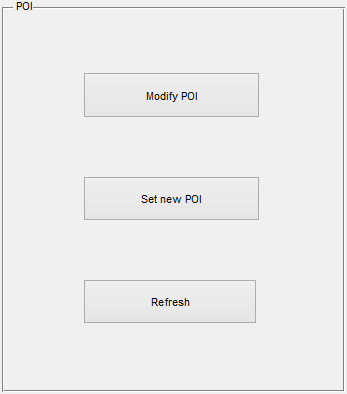
\includegraphics[width=0.4\textwidth]{manipulate_poi}
	\end{figure}};

\node (B) at (-3,-4) [process, text width=5cm, minimum height=0.5cm, align=flush center] 
{\begin{figure}
	\centering
	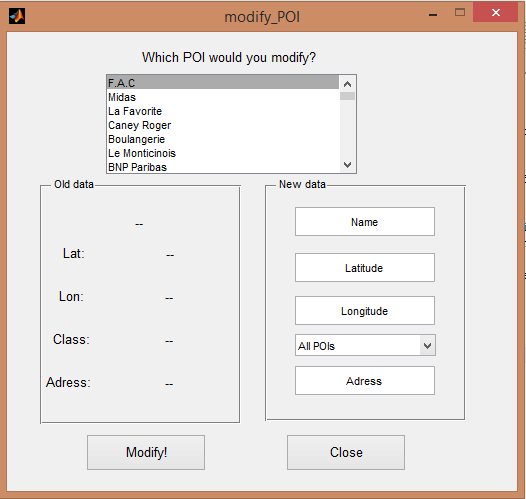
\includegraphics[width=0.8\textwidth]{modify_poi}
	\end{figure}};

\node (C) at (3,-4) [process, text width=5cm, minimum height=0.5cm, align=flush center] 
{\begin{figure}[h]
	\centering
	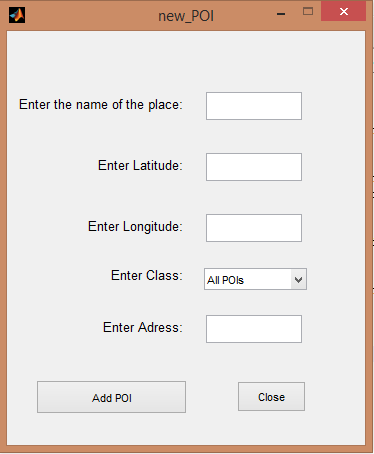
\includegraphics[width=0.8\textwidth]{new_poi}
	\end{figure}};


\draw[->] (-0.6,0.37) -- (-3,0.37) -|  (-3,-2.2);
\draw[->] (0.55,-0.25) -- (3,-0.25) -|  (3,-1.6);

\end{tikzpicture}
\end{frame}

\begin{frame}
\frametitle{Itinerary}
\begin{columns}
	\begin{column}{6cm}
	\begin{itemize}
	\item
	Adding a third point
	\item
	Getting and storing the distance
	\item
	How it works
	\item
	Cost of time
	\end{itemize}
	\end{column}
	
	\begin{column}{6cm}
	\begin{figure}[h]
	\centering
	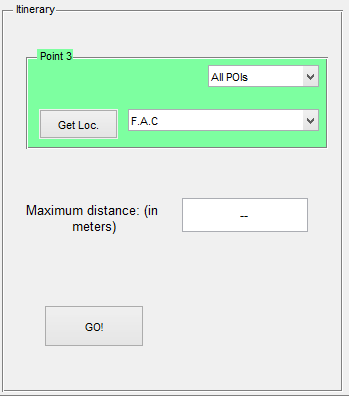
\includegraphics[width=0.8\textwidth]{itinerary}
	\end{figure}
	\end{column}
\end{columns}
\end{frame}

\begin{frame}
\frametitle{Find in a Range}
\begin{columns}
	\begin{column}{6cm}
	\begin{itemize}
	\item
	Using Point 1 data
	\item
	Selection of classes
	\item
	Distance
	\item
	Slow process
	\end{itemize}
	\end{column}
	
	\begin{column}{6cm}
	\begin{figure}[h]
	\centering
	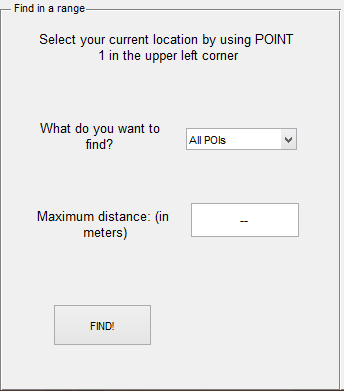
\includegraphics[width=0.8\textwidth]{find_range}
	\end{figure}
	\end{column}
\end{columns}
\end{frame}

\begin{frame}
\frametitle{Generation of the instructions}
\begin{columns}
	\begin{column}{6cm}
	\begin{itemize}
	\item
	Generating instructions from shortest path
	\item
	Setting a scroll bar
	\item
	Exporting this data
	\item
	Default text when missing data
	\end{itemize}
	\end{column}
	
	\begin{column}{6cm}
	\begin{figure}[h]
	\centering
	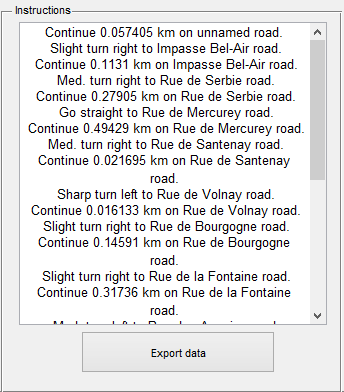
\includegraphics[width=0.8\textwidth]{instructions}
	\end{figure}
	\end{column}
\end{columns}
\end{frame}

\section{Conclusions}
\begin{frame}
\frametitle{Conclusions}

\begin{itemize}
\item
Matlab is more suitable for prototyping and vectorizing operations than C++
\item
C++ deals easier with events produced by the user
\item
C++ allows to export a final released version of the project while to run Matlab program you must have Matlab installed
\item
Performance on C++ implementation is higher but at the same time makes necessary to pay attention to memory leaks
\item
Some functionalities regarding to the GUI are limited in one developing environment but not in other and vice-versa.
\end{itemize}

\end{frame}

\begin{frame}[c]
	\begin{center} 
		\Huge  Thank you for attention! 
	\end{center} 
\end{frame}

\begin{frame}[c] 
	\begin{center} 
		\Huge  Questions? 
	\end{center} 
\end{frame} 


\end{document} 